%
% PROJECT: <ETD> Electronic Thesis
%   TITLE: Looks Good to Me (LGTM): Authentication for Augmented Reality
%  AUTHOR: Ethan Gaebel
% SAVE AS: thesis-draft.tex
% 

\documentclass[12pt]{report}
%\documentclass[12pt,dvips]{report} -- ORIGINAL


\usepackage{graphicx}

\setlength{\textwidth}{6.5in}
\setlength{\textheight}{8.5in}
\setlength{\evensidemargin}{0in}
\setlength{\oddsidemargin}{0in}
\setlength{\topmargin}{0in}

\setlength{\parindent}{0pt}
\setlength{\parskip}{0.1in}

% Uncomment for double-spaced document.
% \renewcommand{\baselinestretch}{2}

% \usepackage{epsf}

\begin{document}

\thispagestyle{empty}
\pagenumbering{roman}
\begin{center}

% TITLE
{\Large 
Looks Good to Me (LGTM): 
Authentication for Augmented Reality
}

\vfill

Ethan D. Gaebel

\vfill

Thesis submitted to the Faculty of the \\
Virginia Polytechnic Institute and State University \\
in partial fulfillment of the requirements for the degree of

\vfill

Master of Science \\
in \\
Computer Science and Applications

\vfill

Wenjing Lou, Committee Chair \\
Ing-Ray Chen \\
Guoqiang Yu 

\vfill

May 15, 2016 \\
Falls Church, Virginia

\vfill

Keywords: 
\\
Copyright 2016, Ethan D. Gaebel

\end{center}

\pagebreak

\thispagestyle{empty}
\begin{center}

{\large Looks Good to Me (LGTM): 
Authentication for Augmented Reality}

\vfill

Ethan D. Gaebel

\vfill

(ABSTRACT)

Augmented reality is a powerful new computer interface paradigm that is going to reshape how people interact with computers. The diverse hardware on typical augmented reality headsets presents an opportunity to the security community to re-make how authentication is carried out, making it more usable for the everyday user and moving authentication away from the cloud and back to face-to-face interactions (when users are face to face anyway). In this paper we explore an authentication protocol to be used when users are face to face and have augmented reality headsets. This protocol uses the same idea behind how humans identify speakers: localizing a wave and comparing its location to a face's location, except here we deal with radio waves instead of sound waves. This protocol is designed to minimize the work required by the user, thus increasing the likelihood that it will be used and decreasing the likelihood of user error. We provide an implementation of the protocol as well.

\vfill

\end{center}

Security-based abstract and stuff!!!

\vfill

% GRANT INFORMATION
This work was supported in part by the National Science Foundation under Grants 
CNS-1443889, CNS-1405747, CNS-1446478, and CNS-1343222.

\pagebreak

% Dedication and Acknowledgments are both optional
% \chapter*{Dedication}
% \chapter*{Acknowledgments}

\tableofcontents
\pagebreak

\listoffigures
\pagebreak

\listoftables
\pagebreak

\pagenumbering{arabic}
\pagestyle{myheadings}

%%%%%%%%%%%%%%%%%
\chapter{Introduction}
\markright{Ethan D. Gaebel \hfill Chapter 1. Introduction \hfill}
% Augmented Reality
% ---- Convince readers it is the future
% ---- Discuss options for AR: headsets, hardware included, etc
% ---- Augmented reality NEEDS a device pairing mechanism
% ---- Why pair point-to-point?
% -------- More efficient network resource usage
% --------- Problem is inherently local
% -------- Not reliant on infrastructure, more robust to patchy areas
% ------------ Cheaper if we consider the non-WiFi usage 
% ---------------- WAY cheaper if you further consider the content size!
% ---- Preserves privacy
% Augmented reality needs device pairing
% ---- Sharing holograms, etc
% Device Pairing
% ---- Difficulty of bootstrapping authentication
% ---- Man-in-the-middle (MOVE)
% ---- Evil twin (MOVE)
% ---- The Resurrecting Duckling (MOVE)
% ---- Long history, briefly summarize to illustrate the breadth of techniques investigated
% ---- Difficulty of pairing over wireless channel 
% ---- Usability's importance to security in practice
% ---- Pin currently dominant method
% ---- Mention centralized device pairing methods.... (this is kind of out of the purview of device pairing; a user account can be used to bootstrap?)
% Augmented reality can have BETTER device pairing
% ---- Improved hardware and user interface provides avenue for BETTER device pairing (better = more usable --> more secure)
% -------- Must be more usable than a pin
% High level description of LGTM from the user perspective (high level even for the user view)
% ---- Press button, look at other person, etc
% ---- Compare EM waves & sound waves for localization & information carrying purposes
% ---- How does this look formally? (transition)


%%%%%%%%%%%%%%%%%
\chapter{Protocol Design}
\section{System Model}
% System Model
% ---- Protocol hardware requirements
% -------- Users have augmented reality head-mounted displays equipped with:
%               wireless communications, support for point-to-point 
%               communications, high resolution cameras, relatively good 
%               computational abilities, and translucent screens very close to 
%               the eye such that only the user can reasonably see them which 
%               are capable of rendering 2D and 3D objects on top of the 
%               physical world which the user is already seeing.
% ---- Users are present, in-person/face to face, and would like to establish 
%           communication to share some kind of content between their devices 
%           which may include: a shared app experience, watching a video, 
%           listening to the same music, shared holograms, basic messaging
% ---- Users of LGTM have no prior security context with regard to their 
%           devices; the users may be friends, acquaintances or strangers.
% ---- Each user possesses, in the memory of their augmented reality headsets, 
%           facial recognition models for themselves.
% -------- These are easily trained via mirror.
% ---- No assumptions regarding access to the Internet are made.

\section{Security Objectives}
% (Security) Objectives
% ---- Authenticate the wireless signal of one user so that secure 
%           communication can be done between two individuals
% -------- Bootstrapping authentication
% ---- Select a user-wireless signal pair to communicate with
% -------- Selection problem
% ---- Privacy Objectives (sub-section under security objectives...)
% -------- No need for centralized power knowing communication/content patterns
% -------- Intermediary parties facilitating communication is 0
% ------------ The potential for remote eavesdropping, censorship, tracking, 
%                   etc, is non-existent

\section{Threat Model}
% Threat Model
% ---- Wireless attacker model

\section{Protocol}
% Protocol, high level (high-level, as in the protocol diagram)

% Protocol Figure
\begin{figure}
\center
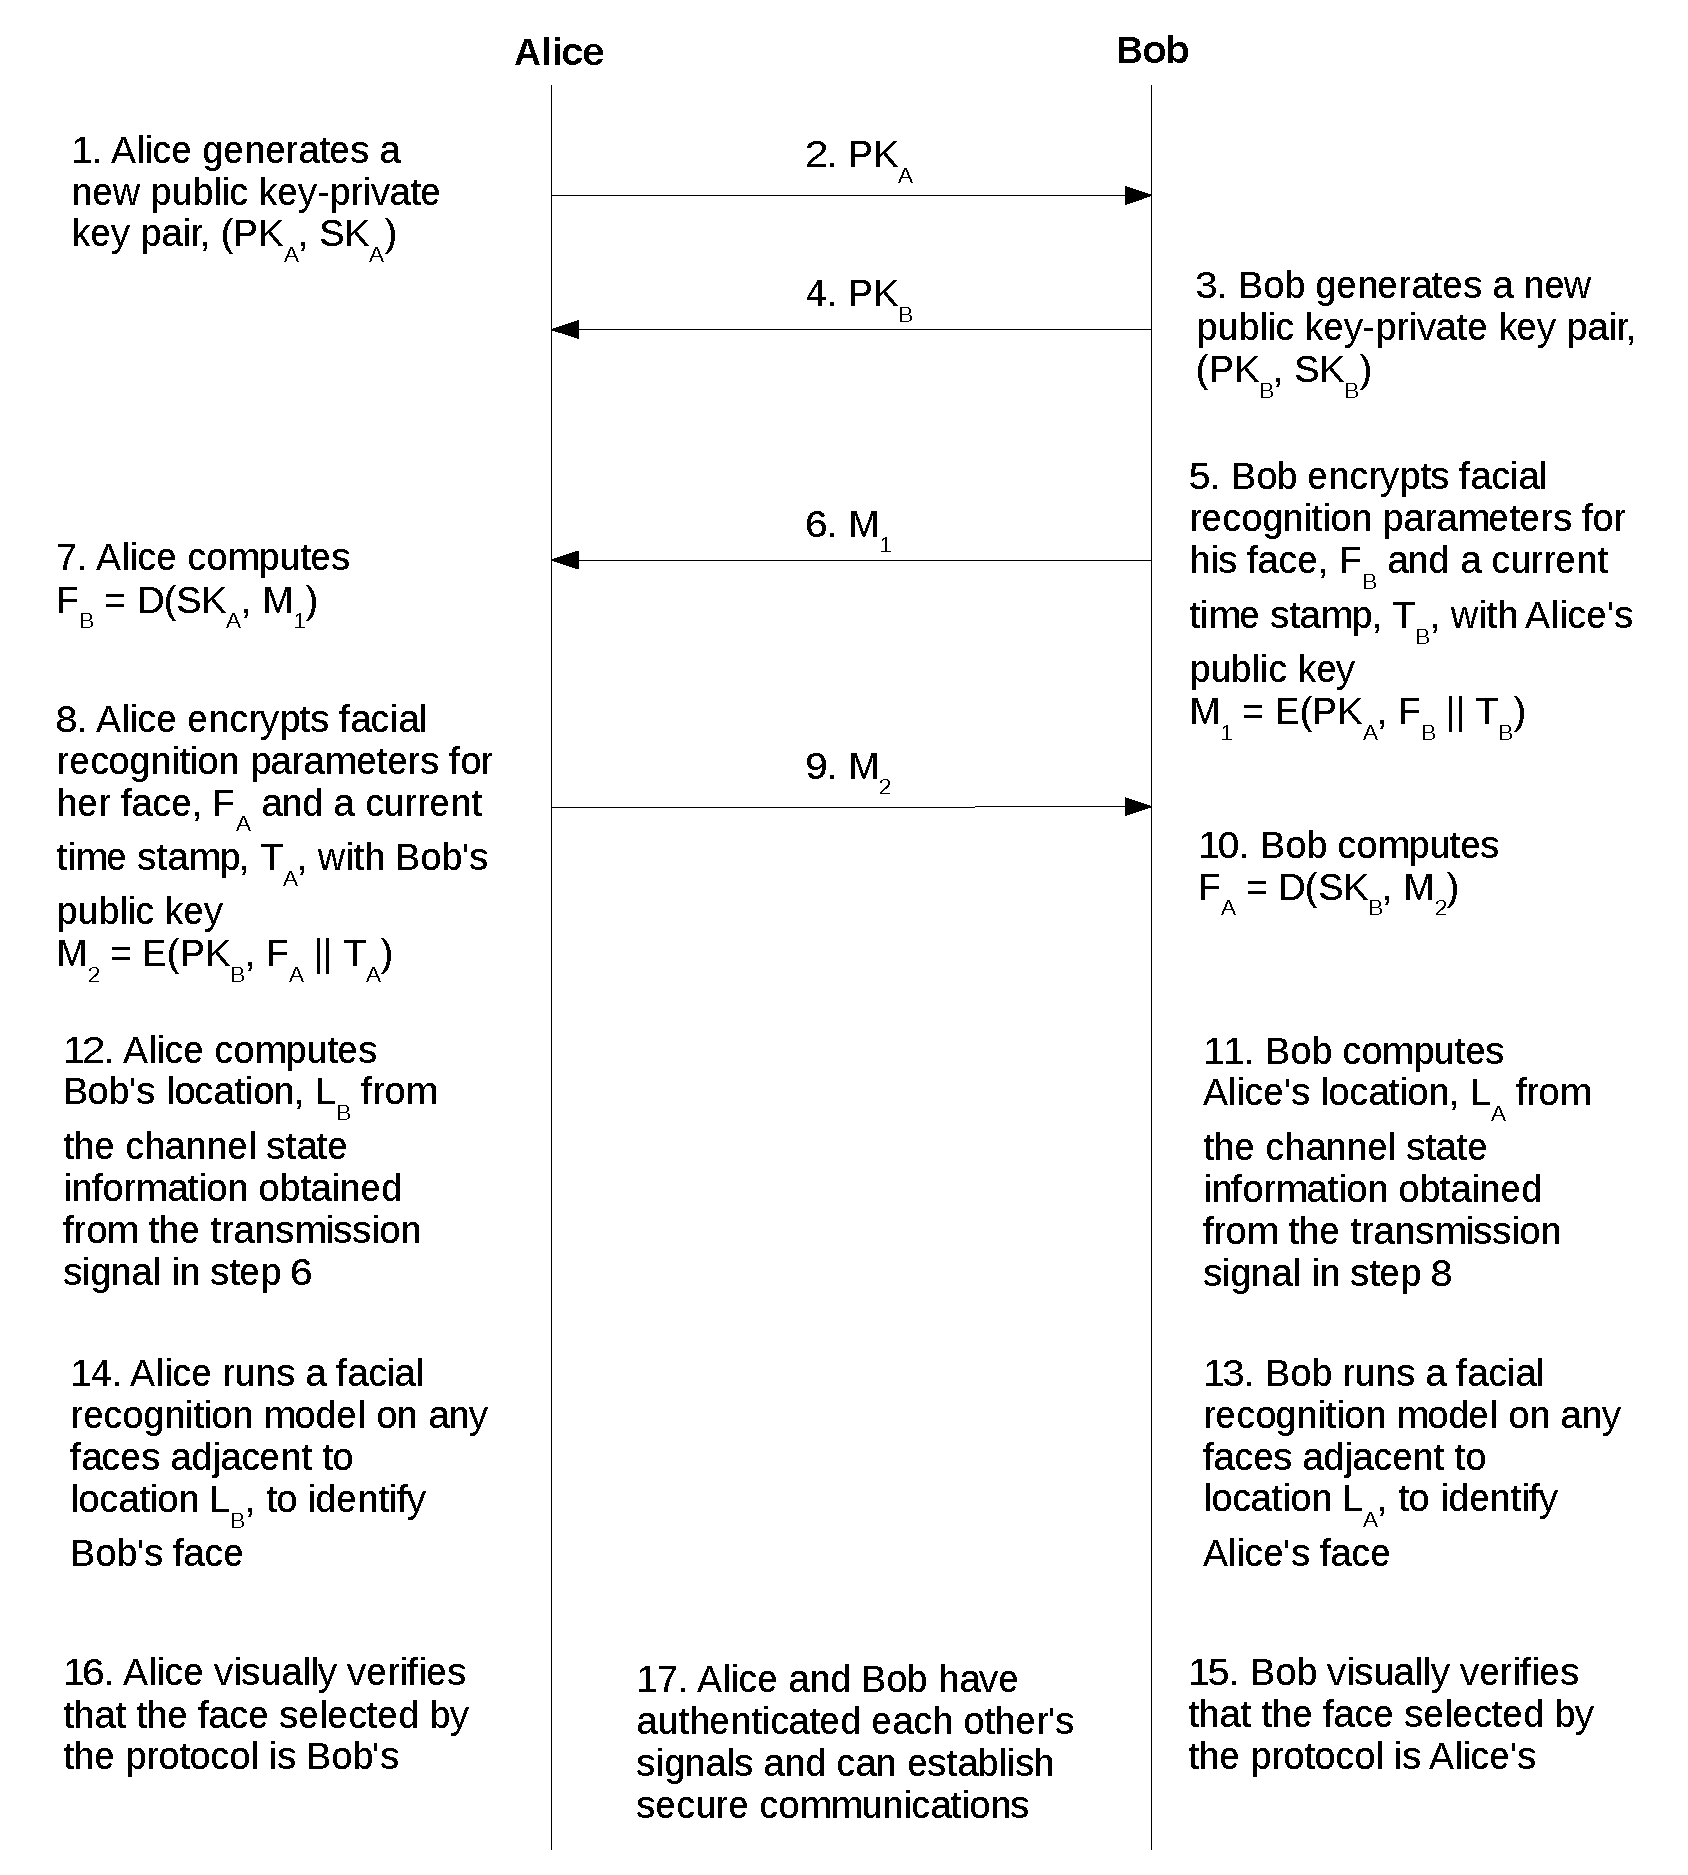
\includegraphics[scale=0.6]{../figures/looks-good-to-me-protocol-diagram--no-legend.pdf}
\caption{Looks good to me protocol diagram...}
\label{protocol-diagram}
\end{figure}

% Protocol, specific (Alice receives $n$ packets, etc...)

\section{Analysis}
% Protocol Analysis
% ---- Describe each step of the protocol (protocol specific above?)
\subsection{Security}
% Security
% ---- Wireless attacks
% -------- Jamming 
% ------------ Works on any wireless pairing technique
% -------- DOS, spam the user(s) with auth requests 
% ------------ Works on any wireless pairing technique
% -------- Man-in-the-middle
% ------------ Works on any wireless pairing technique
% ------------ Wait...the feasibility depends on the quality of the wireless 
%                   localization. In a perfect implementation, this won't work.
% ---- Attacker ability is based on the quality of the facial recognition 
%           & wireless localization (correctness)
% -------- "Attack space" for wireless localization
% ---- Why not a pin?
\subsection{Usability}
% Usability
% ---- Why not a pin?
% -------- Greater range; you can see farther than you can hear
% -------- Will not work in loud environments
% -------- Will not work for the deaf (LGTM won't work for the blind, but 
%                   neither will AR in general, and neither will a pin)
% -------- Depending on implementation, may be less secure, overhearing 
%                   pin can be a security leak
\subsection{Privacy}
% ---- Privacy

\subsection{Potential Alterations}  % Should this section be here?
% Expanding to the group case
% One way sharing: (I.E. Alice receives content from Bob, but not vice-versa)

%%%%%%%%%%%%%%%%%
\chapter{Implementation}
% General setup
% ---- AR headsets unavailable (expensive, not powerful enough yet, not 
%           flexible enough yet)
% ---- Necessary components from AR headsets for experimental purposes (
%           Wireless, video camera, display)
% Wireless Localization Discussion
% ---- Discuss past localization techniques, BRIEFLY
% ---- Discuss lack of focus on point-to-point localization
% ---- Discuss new protocols that enable point-to-point localization in 
%           commodity hardware
% Facial Recognition Discussion
% ---- Very brief discussion of techniques, the area is well studied and my 
%           techniques are not new
% Specific Wireless localization and facial recognition methods
% ---- SpotFi
% ---- OpenCV
% -------- Fisherfaces, LBPH, Haarcascade, etc
% Specific localization & facial recognition components
% ---- Intel 5300 firmware etc
% ---- Laptops with web cams and three antennas each
% System and Validation
% ---- Glue code, system structuring, specifics of protocol implementation
% ---- Explain each implementation decision, why and how, discuss alternatives
% ---- This section should mainly discuss why certain things were NOT done, 
%           and why things ARE done 
% -------- belongs under "General Setup"

%%%%%%%%%%%%%%%%%
\chapter{Experiments}
% Experiments (Very formal)
% ---- Security
% ---- Performance
% ---- SpotFi Accuracy
% -------- Effective "attack space"
% ---- Facial recognition accuracy
% Results (for each above)
% Discussion (for each above)

%%%%%%%%%%%%%%%%%
\chapter{Conclusion}
% List of points to hit on:
% ---- Oldness and difficulty of device pairing
% ---- Usability's impact on security
% ---- Ease of use of LGTM
% ---- Point-to-point communication providing privacy
% ---- Something optimistic and feel-good sounding about the future

%%%%%%%%%%%%%%%%%
%
% Include an EPS figure with this command:
%   \epsffile{filename.eps}
%

%%%%%%%%%%%%%%%%
%
% Do tables like this:

% \begin{table}
% \caption{The Graduate School wants captions above the tables.}
% \begin{center}
%  \begin{tabular}{ccc}
%  x & 1 & 2 \\ \hline
%  1 & 1 & 2 \\
%  2 & 2 & 4 \\ \hline
%  \end{tabular}
% \end{center}
% \end{table}

%%%%%%%%%%%%%%%%%%%%%%%%%%%%%%%%

% If you are using BibTeX, uncomment the following:
% \thebibliography
%
% Otherwise, uncomment the following:
% \chapter*{Bibliography}

% \appendix

% In LaTeX, each appendix is a "chapter"
% \chapter{Program Source}


\end{document}